\part{Analysis}
		\chapter{Introduction}
		Before creation of the main product can begin, an understanding of the relevant fields must be achieved. The first aim of the analysis is to develop this understanding, by evaluating and then understanding relevant literature that has been identified as being relevant to the project. Following this appropriate tools for the product will be identified, both hardware and software. Finally conclusions will be drawn based on what has been researched and evaluated, and a series of core objectives that need to be achieved for the project to be a success will be determined. The achievement of these objectives should be possible thanks to the research that will be carried out here.
		
		
		\chapter{Mobile Robotics}
			\section{Introduction}
			Here we will address some of the key aspects of mobile robotics that are relevant to the project, chiefly how movement is dealt with in mobile robotics as well as range-finding.
			
			\section{Movement}
			This section aims to explore how movement is generally achieved in the world of mobile robotics. From this, a greater understanding of robotic movement should be achieved which will aid the robot's development.
			
				\subsection{Chassis}
				Most conventional vehicles use standard wheels that have only two degrees of freedom. These wheels can either roll forwards or backwards. This means it is a non-holonomic vehicle, which essentially means at any given point in the vehicle's state there are certain directions it cannot travel in. This can present a few problems. Firstly, navigation will sometimes involve the adjustment of the vehicle's heading. The vehicle may need to reverse and turn before it can move forward to a certain location. This presents a problem in the robot's efficiency and ability to navigate around a difficult environment, as well as making it more challenging to implement from a software perspective as we would need to factor in situations where these sorts of adjustments would be needed before the robot can proceed. If the robot were to be holonomic however, then it would be able to begin travelling toward any location regardless of its current position. This can be achieved if the wheels our robot's chassis uses are omni-directional.	
				
				Watanabe\citep{watanabe1998control}, a Professor at Okayama University's Faculty of Engineering who has published a great deal of work in robotics, discusses a few different variations of these omni-directional wheels. One of the more popular variations in his discussion is the universal wheel, sometimes also referred to as the swedish wheel or mecanum wheel. This wheel is a larger wheel that has many rollers on the rim which allows the wheel to slide in a direction perpendicular to its motor axis. 
				
				\begin{figure}[h]
					\centering
					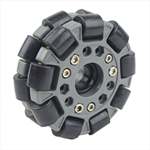
\includegraphics[width=.3\linewidth]{ANALYSIS/90degwheel.png}
					\caption{An omnidirectional wheel, with 90 degree rollers}
					\label{90 Degree Omni Directional Wheel}
				\end{figure}
				
				A robot chassis composing of three or four of these wheels as well as relevant motors should be adequate. A few of the different chassis found during the preliminary research will now be evaluated to find which would be the most suitable for the project.
				
					\subsubsection{4WD 58mm Omni Wheel Arduino Robot - \pounds{260.78}}
					\begin{figure}[h]
						\centering
						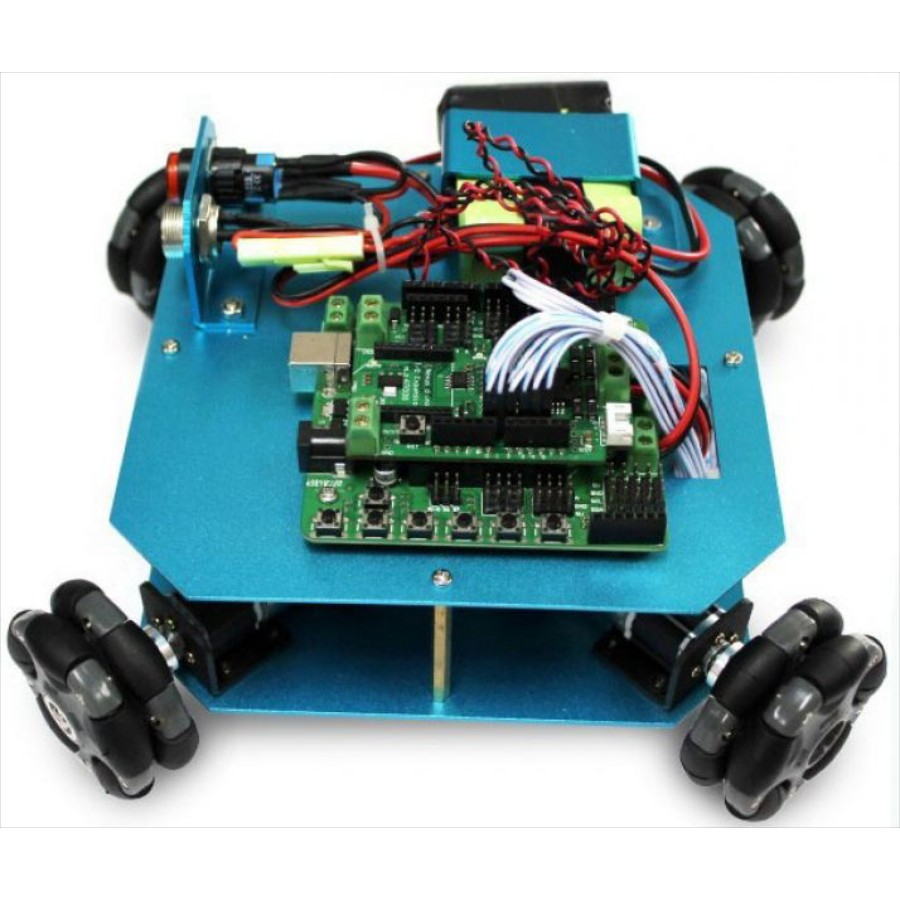
\includegraphics[width=.3\linewidth]{ANALYSIS/4wdomnidirectionalarduino.jpg}
						\caption{4WD Omni-Directional Robot Chassis}
						\label{4WD Omni-Directional Robot Chassis}
					\end{figure}
					This chassis features four of the aforementioned omnidirectional wheels along with appropriate motors. The motors have encoders with them which record wheel revolutions, allowing us to use odemetric measurements should we connect these encoders to the microcontroller. This kit includes the microcontroller which is an Arduino 328, as well as a nickel metal hydride battery and an appropriate charger. The kit also includes an IO expansion board which would allow us to connect more external devices. 
				
					Whilst it would be useful to have most of the equipment decisions done for us, some of this is not necessary. The IO expansion board for example will most likely be needed, as all we're really interested in adding is a sensor for observations. As well, the price of the kit is quite high given we would also need to purchase a LIDAR sensor on top of it.
				
					\subsubsection{3WD 48mm Omni-Directional Triangle Mobile Robot Chassis - \pounds{114.34}}
					\begin{figure}[h]
						\centering
						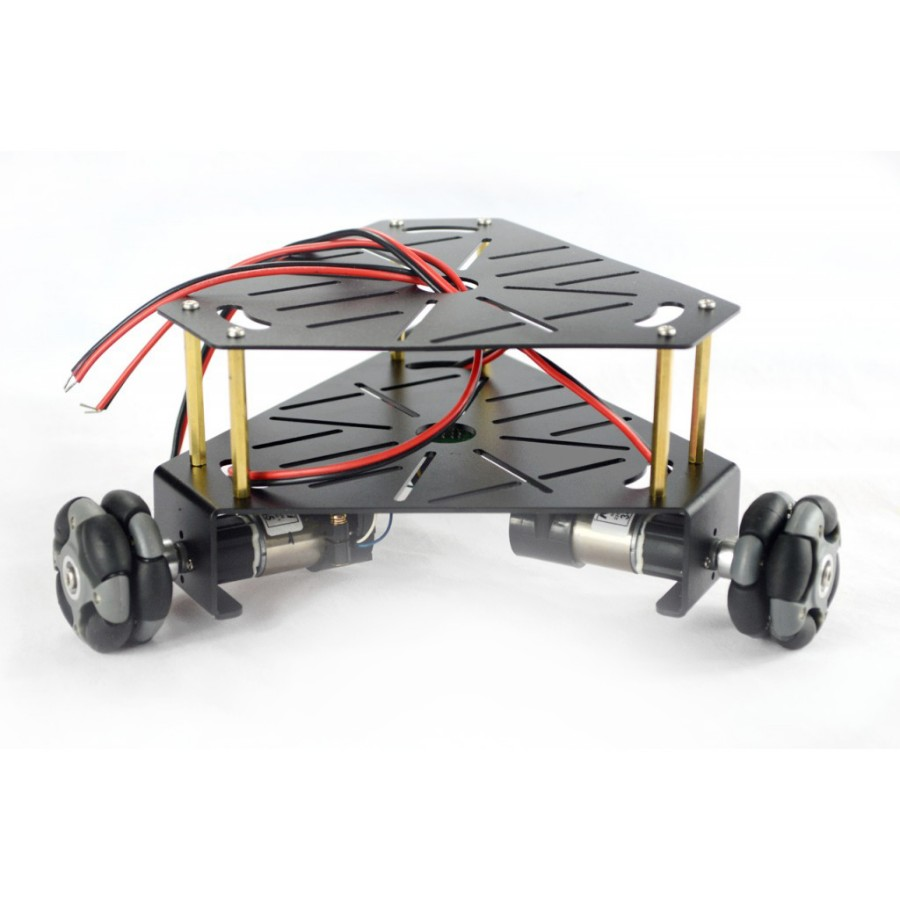
\includegraphics[width=.3\linewidth]{ANALYSIS/3wdomnidirectionalchassis.jpg}
						\caption{3WD Omni-Directional Robot Chassis}
						\label{3WD Omni-Directional Robot Chassis}
					\end{figure}
					Unlike the previous chassis this one features only three wheels rather than four. This is still enough to achieve freedom of movement however. Whilst it doesn't include the additional pieces of the kit the other does (such as a microcontroller) we still have our wheels, a supporting structure and appropriate motors with encoders that will provide us with odometric data. There is plenty of room in the middle for items such as our microcontroller and a power source, and the top plate is an ideal mounting point for our sensor.
					
					Whilst still a bit expensive, the chassis is still on the cheaper side compared to the previous one and some cost is expected to be incurred given that a 12v DC motor with an encoder can cost around \pounds{30}. One issue encountered while looking for an appropriate robot chassis is that the majority on sale seem to already include microcontrollers and sensors, which launches their price up and also removes a lot of the choice from the product. Looking around the RobotShop and HobbyTronics website for just an empty chassis only yielded this product. Based on these factors, this chassis will be the one used for the product.
					
					
			
			\section{Rangefinding}
			To achieve self navigation as well as mapping, the robot will need to take observations about its surrounding environment. In order to efficiently map the area and detect obstacles this will need to be performed in a 360 degree manner as well. This sections aims to explore a few of the most common approaches to rangefinding.
			
				\subsection{Infrared}
				Infrared sensors work by measuring things via the reflection of infrared light. The sensor will send out some infrared light where it will be reflected off of an obstacle. A reciever will capture this reflected light and depending on factors such as how much light is recieved back and the triangulation of how the light was recieved the presence of an obstacle will be determined. There are a number of Infrared sensors available online for very cheap prices, websites like RobotShop and HobbyTronics list most of their sensors between £5 and £10. 360 sensors are incredible difficult to find, but their low price means purchasing a few would not be a problem.
				
				The range and degrees of space being measured will depend on the sensor's model, but there are a few things the different sensors have in common. First, infrared sensors have both a maximum and a minimum range. Not only does the maximum range need to be factored in as sensor will struggle to pinpoint the location of light that has been reflected at a large range, but the sensor will also struggle to 'see' very close obstacles. In addition, infrared sensors struggle in strong sunlight and seem best suited to primarily indoor tasks.
				
				
				\subsection{LIDAR}
				LIDAR (Light Detection And Ranging) is a technology that uses light sensors to measure distances between the sensor and the target object. It achieves this by sending out light pulses which bounce off of objects back at the sensor where they are collected.
				
				LIDAR has seen some popularity in mobile robotics and the decision to use LIDAR would give the project some interesting options. Some sensors boast very impressive statistics, with some ranges exceeding 10 metres whilst providing several thousand samples per second with 360 degree coverage \citep{slamtecA1M8}. Some of these sensors also feature SDKs (Source Development Kits), meaning the core sensor functionality will be accessible straight away allowing development to focus on the robot's logic rather than being bogged down in the belt and braces implementation of preliminary functionality. These features are expensive however, with some sensors being as high as \pounds{350}.
				
				\subsection{Ultrasonic}
				Ultrasonic sensors function by sending out ultrasonic pulses and measuring the amount of time it takes for these pulses to bounce back. Because sonar is sound based rather than light based, it isn't negatively affected by aspects such as heat, colour or dust. Sensors can interfere with each other however, sonar sensors sending and receives pulses in close proximity to each other can cause issues. A single robot is only being developed, but given that we may need multiple sensors to perform a full 360 degrees of observation this could cause some considerable complications. Sonar sensors can be found relatively cheap depending on the sensor, with sites like HobbyTronics and RoboShop featuring sensors as cheap as \pounds{6} ranging up to some that cost around \pounds{50}.
				\medskip
				
				it would appear that LIDAR, whilst the most expensive option, is what will provide the project with the most functionality and ease of use. Here we will look at a few different LIDAR sensors that could be suitable for the project.
				
				\subsubsection{RPLIDAR A2M8 360 Degree Laser Scanner - \pounds{301.43}}
				\begin{figure}[h]
					\centering
					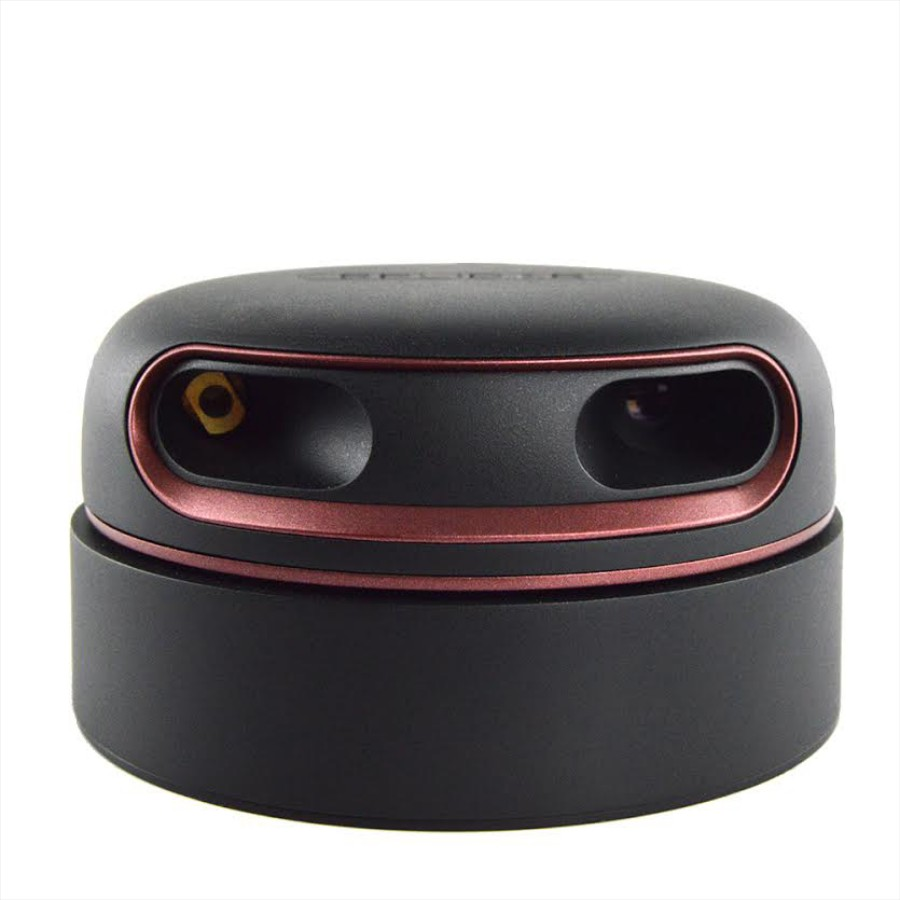
\includegraphics[width=.3\linewidth]{ANALYSIS/rplidara2.jpg}
					\caption{RPLIDAR A2M8}
					\label{RPLIDAR A2M8}
				\end{figure}
				The RPLIDAR A2M8 uses the previous described LIDAR triangulation system, and outputs scan data at 8000 samples per second\citep{rplidarm8docs}. It outputs this data via a relevant communication interface, representing scans as distance (what distance between the sensor and the measuring point) and heading (the heading angle of the measurement). It also includes a start flag in its measurement signalling the start of a new scan, which would likely come in useful for processing the scan data as we could simply check this flag to see if incoming data is from a new scan. One of the biggest advantages to employing this sensor would be the SDK it comes with. With full documentation, the SDK allows us to access the sensor's entire functionality straight away. It has appropriate methods for beginning the scanning session, ending it and checking sensor health as well as a few other things. This would save a lot of time in the project as we could focus on logical implementation rather than creating the prerequisites that will be needed for the sensor to do what we need it to do.
				
				The major downside to all of these advantages however is the cost. Sitting at just above \pounds{300}, this is an incredibly steep price for the project if we factor in the cost of the other equipment such as the chassis. This problem leads us to the final choice.
				
				\subsubsection{RPLIDAR A1M8 360 Degree Laser Scanner - \pounds{93.54}}
				\begin{figure}[h]
					\centering
					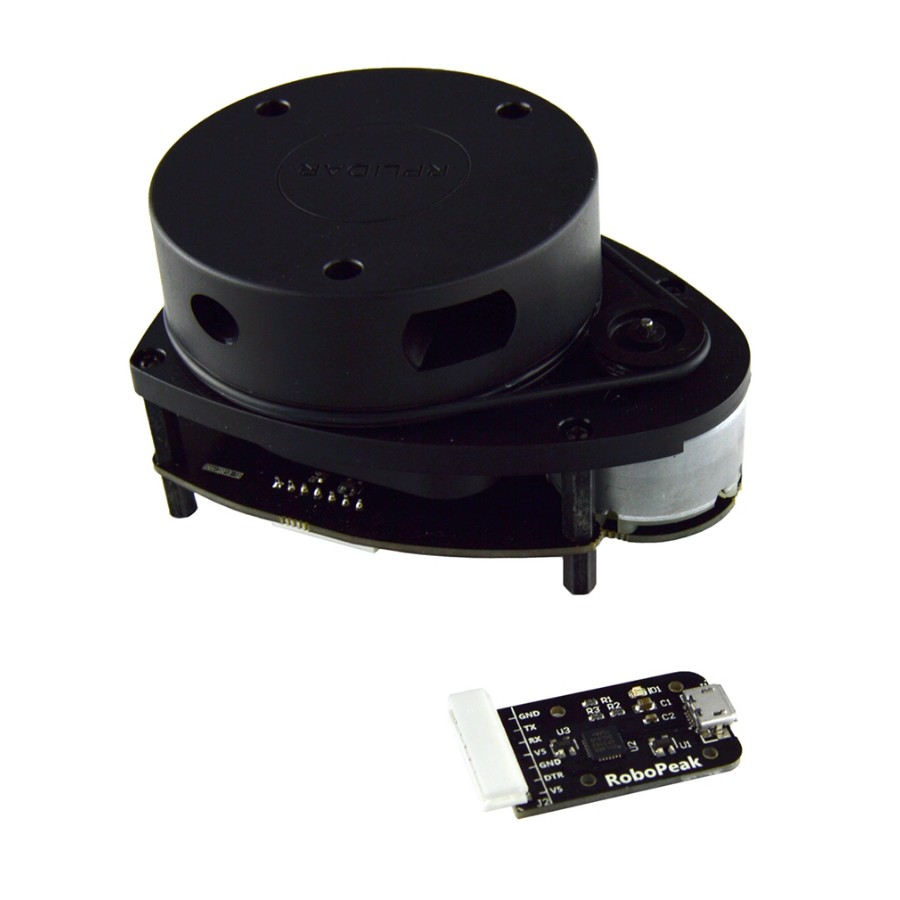
\includegraphics[width=.3\linewidth]{ANALYSIS/rplidara1.jpg}
					\caption{RPLIDAR A1M8}
					\label{RPLIDAR A1M8}
				\end{figure}
				Essentially a less sophisticated version of the previous sensor, this iteration of the M1 LIDAR sensor still offers us a 4000 - 8000Hz sample frequency as well as the previously mentioned SDK. Among a few other things, the key differences here are that we have a slightly slower scan frequency (1 - 10Hz vs the A2's 5 - 15Hz) and a few pieces of SDK functionality that aren't available on the less advanced firmware. The key change is that we lack the express scan function, which is similar to the regular scan but it performs at the highest sampling rate the sensor can use. 
				
				These downsides are negligible with our product however, ultimately as long as we can easily get observational data at a reasonable rate the project benefits hugely. This functionality at the far more agreeable price point makes this the sensor of choice for the robot.
				
			
		
		\chapter{An Investigation Into SLAM}
			\section{Introduction}
			The development of a moving robot is only one half of the end product. As previously mentioned in the project's Terms of Reference the purpose of this project is also to develop a robot that is capable of self navigation and mapping. In order for this to be possible, the robot must be capable of using observations about its environment to build a map. Not only that, but it also must track its own location within this environment. This chapter aims to explore SLAM, a computing problem with research and implemented solutions that deal with exactly that.
		
			\section{What is SLAM?}
			SLAM stands for Simultaneous Localization and Mapping, and is something sometimes employed by mobile robots. Localization refers to the ability for the robot to be aware of its location within an environment, for example knowing where it is within a room. Mapping simply refers to building a map of the environment, such as the room the robot is in. SLAM is performing both of these tasks at the same time. Durrant-Whyte and Bailey\citep{durrant2006simultaneous}, both academics that have done extensive work in the field of mobile robotics, best sum it up as the ability for a mobile robot to be placed at an unknown location in an unknown environment and then both create a consistent map of the environment and be able to accurately determine its location within this map. Similar definitions can also be found in other articles \citep{choset2001topological, dissanayake2001solution}.
		
			\section{Uses of SLAM in Industry}
			There are a myriad of potential uses for SLAM, many of which can be seen within the wider industry. Commercially it has been used for products such as vacuum cleaners, Dyson for instance has a small automated vacuum cleaner called the 360 Eye which employs SLAM techniques to map the areas that it moves around and cleans. SLAM has seen many uses in archaeological contexts owing to its ability to perform exploration without risk to human life, one team \citep{clark2008archaeology} developed an underwater robot that used SLAM in order to map underwater cisterns that had been built thousands of years ago. The uses have not gone unnoticed by larger organisations. One of the research organisations within the USA's Department of Defense has held challenges (known as the DARPA Grand Challenge) offering cash prizes as incentives to create high value research. These challenges involve organisations submitting cars that are timed as they race around certain environments. NASA have also made use of it in the past, in 2007 they used an autonomous underwater robot \citep{carnegie2007sinkhole} employing SLAM to go to the bottom of the world's deepest sinkhole. The robot used sensors to generate a sonar map of the sinkhole's inner dimensions 318 meters below the surface.  The drone also tested technologies that could be used in other more extreme underwater environments such as the oceans under the crust of Europa, one of Jupiter's moons. This has led to increased interest being expressed in using SLAM for planetary rovers, which would allow for the mapping and navigation of different planet surfaces.
			\medskip
		
			\section{The SLAM Problem}
			Let's use some key notations to help break down the essentials of the SLAM problem. \newline
			\textbf{t} - Current time. \newline
			\textbf{x\textsubscript{t}} - Location and orientation of vehicle. \newline
			\textbf{u\textsubscript{t}} - Control vector, for example drive forward 1 metre.  \newline
			\textbf{m\textsubscript{t}} - True location of \textit{i}th landmark within the environment. \newline
			\textbf{z\textsubscript{t}} - Observation of \textit{i}th landmark taken at time \textit{t}.\newline
			
			From these notations we can derive some sets. \newline
			\textbf{x\textsubscript{0:t}} = $\lbrace$ \textbf{x\textsubscript{0:t-1}}, \textbf{x\textsubscript{t}} $\rbrace$ - History of all vehicle locations. \newline
			\textbf{u\textsubscript{0:t}} = $\lbrace$ \textbf{u\textsubscript{0:t-1}}, \textbf{u\textsubscript{t}} $\rbrace$ - History of odometrical information pertaining to teh robot's movement. \newline
			\textbf{m} = $\lbrace$ \textbf{m\textsubscript{1}}, \textbf{m\textsubscript{2}}, ..., \textbf{m\textsubscript{n}}$\rbrace$ - Set of all landmarks. \newline
			\textbf{z\textsubscript{0:t}} = $\lbrace$ \textbf{z\textsubscript{0:t-1}}, \textbf{z\textsubscript{t}} $\rbrace$ - Set of all landmark observations. \newline
			
			Ultimately we want to use the robot's control inputs and observations to receive a map of the environment and the robot's path.
			
			\begin{figure}[h]
				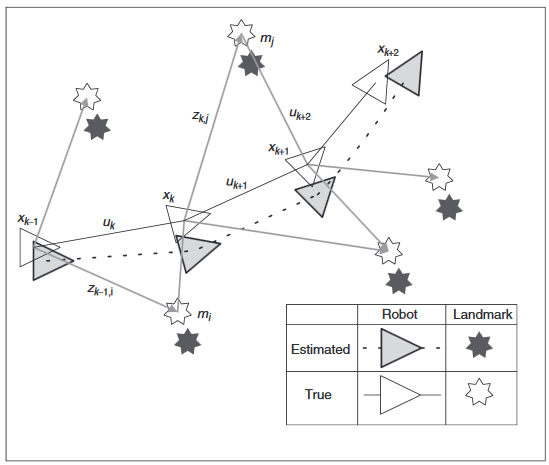
\includegraphics[scale=0.65]{ANALYSIS/slamdiagram.png}
				\caption{The SLAM problem illustrated \citep{durrant2006simultaneous}}
				\label{fig:slamillustration}
			\end{figure}
			
			SLAM is generally approached probabilistically. This means that the attempted solutions factor in uncertainties within the data. Therefore, solutions to the SLAM problem will not act with exact certainties. For example, rather than saying the robot is in an exact location we would treat it as a general location it is the most likely to be in. We want the probability distribution to be an estimation of current vehicle location and landmarks based on landmark observations and control inputs or odometrical data. 
			
			There are variations within the SLAM problem however. At a broader level, SLAM problems generally come in one of two flavours. These are full SLAM and online SLAM. 

				\subsection{Full SLAM}
				Full SLAM involves using landmark observations and data relevant to discerning the robot's current position in order to determine the robot's entire path. It can be written as such -
				
				p(\textbf{X\textsubscript{0:t}}, \textbf{m} $\mid$ \textbf{Z\textsubscript{0:t}}, \textbf{U\textsubscript{0:t}})
				
				\subsection{Online SLAM}
				Online SLAM differs slightly in that it seeks to determine the robot's current location rather than the robot's entire path. It can be written as such - 
				
				p(\textbf{x\textsubscript{0:t}}, \textbf{m} $\mid$ \textbf{Z\textsubscript{0:t}}, \textbf{U\textsubscript{0:t}})
				
				\subsection{SLAM Taxonomy}
				The possible differences in the SLAM problem don't end there. Depending on different factors there are also different sub approaches to the SLAM problem. Below are some common variants.
				
					\subsubsection{Volumetric versus Feature-Based}
					Volumetric SLAM samples the map as a resolution high enough to allow a photo realistic reconstruction of the environment \citep{thrun2008simultaneous}. The map gained from this is generally high dimensional, but as the area increases in size and scale the map becomes significantly more complex. Feature-based SLAM simply extracts key features from measurements, with the map being solely made up of these features. This might be used if it is decided that only key features are of interest or if large parts of the mapped space are empty, as volumetric SLAM in these cases would be storing voxels that hold no geometric data of significant value \citep{vespa2018efficient}. As you would expect, this is quicker and more efficient but discards a lot more data than volumetric. 
					
					\subsubsection{Topological versus Metric}
					Topological SLAM captures key places and their connectivity to other measured locations. Metric SLAM attempts to model the environment using geometrically accurate positioning. Metric SLAM would show the accurate positioning of various environmental features, topological would show them in relation to each other (e.g. place A is adjacent to place B) \citep{thrun2008simultaneous}. A good analogy would be a bus route map (topological) that displays the different stops versus showing the bus' actual route on a geographical map of the area (metric).
					
					\subsubsection{Known versus Unknown Correspondence}
					This entails relating the identity of sensed landmarks to other sensed landmarks. In known correspondence the identity of the landmarks is known, if a landmark is observed and then the robot moves and observed another landmark, the identity of the landmarks being known would let us to determine if this landmark observation is the one we saw before or a newly observed one. Unknown correspondence would simply mean that in this situation we wouldn't know.	
					
					\subsubsection{Static versus Dynamic}
					Static and Dynamic here refers to the environment. Static SLAM algorithms assume that no changes will take place in the environment whereas Dynamic SLAM methods allow for these changes to take place.
					
					\subsubsection{Small versus Large Uncertainty}
					The ability to represent uncertainty is another aspect. Some SLAM approaches will assume a very low uncertainty in the robot's location estimation. This might be when the robot is moving up and down a simple path, as it's much easier to guess where it's likely to be. Large amounts of uncertainty might occur however in more complex environments where locations can be reached from multiple different directions, or if the robot starts travelling in more complex paths that intersect with each other.
					
					
					\subsubsection{Activate versus Passive}
					Active SLAM involves the robot actively exploring its environment whilst it builds a map of it. Passive SLAM is when the SLAM algorithm is purely used for observation, with some other entity controls the robot's movement. 
					
					\subsubsection{Single-Robot versus Multirobot}
					Single-robot simply refers to SLAM happening only on a single platform. Multirobot SLAM (sometimes known as cooperative SLAM) involves multiple robots often communicating with each other to merge their maps into a larger collective model. 
				
					\medskip
					There are multiple different paradigms that can be used to solve the SLAM problem, and each of these paradigms has many different implementations. One technique that has seen usage for solving the SLAM problem in autonomous mobile robotics is the Canonical Scan Matcher, generally referred to as CSM. This is the solution that we will be looking to implement for the project.

			\section{A Look At A Potential Solution}
				\subsection{Introduction}
				As previously discussed there are a myriad of variations on the SLAM problem, and there are a few different paradigms used to implement solutions to it. During some preliminary research, one method of SLAMming came up that seemed like it would be suitable for the project called CSM.
				
				\subsection{CSM}
				CSM is an open-source C implementation of an ICP variant known as PlICP. It has seen usage for industrial prototypes of autonomous robotics, one of the most notable examples of this being Kuka, a German manufacturer of industrial robotics. It isn't quite a fully fledged SLAM solution, instead performing pairwise scan-matching on scan data that is fed into it. Before the PlICP algorithm it is based on can be explained, we must first look at the base ICP algorithm.
			
					\subsubsection{ICP}
					ICP stands for Iterative Closest Point, and it refers to an algorithm that attempts to minimize the difference between two clouds of points, something known as point matching or point set registration. In essence, it means getting one set of points aligned to another set of points. Besl and McKay present the algorithm as a statement \cite{besl1992method} in their paper, and ICP is shown in terms of C++ in the Mobile Robot Planning Toolkit \citep{mrpt2013icp}. 
					
					We first of all have a source map, and then we have a map that we wish to align to it which we will refer to as the reference map. We then go through each point in the source map and which point in the reference map is the closest to it. We then determine a transformation which would minimize the mean squared error (the average squared difference) between the two points before applying this transformation to the reference set and then going through this set of steps again. This is repeated until a the mean squared error falls below a certain threshold.
					
					\subsubsection{PlICP}
					Censi explains PlICP in a series of steps \citep{censi2008icp}. To start with, we take a reference scan, a second scan and a first guess for the translation needed to try and match the two maps. We then generate a polyline of the reference map by connecting sufficiently close enough dots (using a threshhold). Following this, a loop similar to the one in the base ICP algorithm begins.
					
					We first determine the coordinates of the second scan in the first scan's frame of reference using our initial translation guess. Then, for each point in the second scan, we determine the two closest points to it in the first scan. We trim any outliers within these matches, and use the sum of the squares of the distances from the points to the line containing the matches two points to find the error function. PlICP then uses an algorithm in order to minimize this error function which we now use as our translation guess. This new guess is used on the next iteration of the algorithm. This loop continues until either we have a convergence between the maps or a loop is detected as no further progress is being made.	
					
			\subsection{Suitability of CSM}
			Firstly we can see that CSM is a pure C implementation of the previously described algorithm. This is excellent for the project, not just for the benefits of C such as it being a relatively quick language but also because it should be directly usable with an embedded board which would be the ideal choice for controlling the robot. Had it been in any other language we might have needed to use some sort of shared library to get it to work which likely would have slowed things down and potentially made the robot less effective. 
			
			CSM is however not a product of a professional company dealing in these matters, its open source nature could put some doubts with regards to its usefulness or reliability. However, it was developed by Dr Andrea Censi, someone who is a Deputy Director for the Chair of Dynamic Systems and Control at ETH Zurich meaning it is far from an amateur project. As previously mentioned as well it has been adopted by the German robotics company Kuka, so clearly it has enough merit to be used at the industrial level. Ultimately it would appear CSM is an ideal choice for the robot's localization and mapping functionality.
					
			\section{An Investigation Into SLAM - Conclusions}	
			First and foremost we can safely establish that the SLAM problem is what we are addressing with regards to the implementation of the robot's ability to track its own location whilst mapping its environment. In addition to this we understand the fundamentals of the SLAM problem. This will massively benefit development, as being aware of having to store details internally such as wheel revelations gained via odometric sensors will allow us to cut down on time spent during development having to rewrite core pieces of functionality to make room for this. 

		%\chapter{Solutions}
		
		
		\chapter{Review of Tools and Techniques}
		
			\section{Dealing with Scan Data}
			One aspect that needed to be considered was the drone's behaviour whilst scanning. The initial thought was that the drone would move around, scan and save the scan results all simultaneously. To investigate the viability of this tests were performed to see if this was possible with the constraints we had, the most notable constraints being how quickly the MBed board is able to write scan data compared to how quickly it would be receiving it from the LIDAR sensor. Based on this it was decided it would be best if the LIDAR stopped and took readings for a small period of time, with these readings being stored in the RAM and then written to internal files afterward. 
			%*!Have some numbers here describing the time it takes to write data retrieved from 1 seconds' worth of LIDAR scanning!*
			
			
			% QUESTION -- is it worth talking about dead reckoning when we aren't using it for the actual product?
			\section{Dead Reckoning}
			Odometry is the usage of data from motion sensors to estimate an object's position. One such implementation of this that will be looked at for the project is dead reckoning. Dead reckoning tracks the robot's position by using data from wheel encoders that count the number of wheel rotations performed during operation. From this, the internal tracked position of a robot can estimate its new position after periods of movement. Given that the chassis being used for the project has wheel encoders as part of the wheel motors, this approach would allow us to perform odometry without needing the use of additional kit. Dead reckoning is not without issues however. Most pressingly it does not account for wheel slippage. If the robot has a poor grip on the ground and the wheels slip, then the wheel rotation doesn't accurately correspond to the robot's location \citep{choset2001topological}. These issues would compound as well. As more and more slippage happens, the robot's internal position would become less and less accurate to where it actually is. 
		
			\section{Software Framework}
			With regards to the software that will be running on the robot itself, it makes sense to implement it as an operating system. Appropriate tasks will be made to deal with things such as the robot's movement and interaction with the LIDAR sensor. This section aims to explain our potential options for how this operating system will be implemented before coming to a conclusion on which of the options will be used and why.

				\subsection{MBED RTOS}
				The MBED Real-Time Operating System is an open source operating system for platforms using Arm microcontrollers. It is specifically designed for IoT (Internet of Things) devices, which the OS documentation\citep{mbedrtosdocs} define as low-powered, constrained devices which require access to the internet.
			
				Aside from the usual features you'd expect from an operating system (threads, semaphores, etc), MBED OS also features C++ based network sockets for the sending and recieving of data, network interface APIs for interfacing with things such as ethernet or wi-fi as well as bluetooth support. One aspect of the Terms of Reference dealt with precisely how map data would be handled, with two of the three options involving wireless transmissions. Should the project go in this direction, MBED OS' numerous APIs for dealing with this would be immensely helpful. All of this may be overkill however, communication without the use of these APIs isn't impossible and if we don't use wireless communication then all of these features will be of no use anyway. Should another method of dealing with map data such as locally storing it, a much simpler OS would be more appropriate.
				
				\subsection{\textmu C/OS-II}
				\textmu C/OS-II (which will hereon be referred to as Micro C OS) is a very simple real time operating system designed for use with embedded systems. Labrosse\citep{labrosse2002microc} discusses a number of different features of Micro C OS in the documentation in addition to ones you would typically find in an operating system (semaphores, task management, etc). Labrosse discusses how Micro C OS is able to be used on a wide variety of microprocessors owing to its design, allowing it to be highly portable. In addition, Micro C OS's scalability is discussed, allowing for only the services required in the operating system's host application to be used. This feature in particular would come in useful for the project given the use of a microcontroller, as it would allow us to cut down memory usage to only what we need which should help performance issues from arising.
				
				% where should this go?
				\subsection{Microcontroller}
				
		\chapter{Conclusions}
		%Look at the objectives from the TOR, outline what the robot and the software needs to do to achieve these objectives.
		Based on the different aspects of mobile robotics and SLAM that have been looked at as well as the critique of the various tools and techniques that have been employed, we can outline the basic product requirements that will need to be achieved in the course of the product's development. First and foremost the robot must be capable of basic navigation. The drone must be capable of observing the environment using rangefinding techniques. Finally, the robot must be capable of processing data acquired through this rangefinding process to perform localization and mapping. Finally, the retrieved observational data must be processed and fed into the CSM software to generate a map. For this to happen the robot needs to be able to somehow store the observational data it retrieves from the LIDAR sensor, and we also need a medium to put the data into CSM and display the output. From this outline we can get these basic project requirements -
		
		\begin{itemize}
			\item The robot must be capable of movement
			\item The robot must be capable of observation
			\item The robot must be capable of storing observational data
			\item The observational data must be processed into a map
		\end{itemize}
	
	
	
		
				
	